\subsubsection{Propósito}

\subsubsection{Arquitectura}

\subsubsection{Aspectos técnicos generales}

Se debe aclarar que \textbf{VMWare ESXi} es software privativo, se debe adquirir una licencia para poder utilizarlo comercialmente. Para el presente trabajo se utilizan versiones de prueba de la herramienta. También es importante tener presente que para poder acceder a dichas versiones es necesario crear previamente una cuenta de usuario gratuita en el sitio web de VMWare (Ver figura \ref{fig:VMwareInstalacion01}).\\

\begin{figure}[!hbtp]
	\centering
	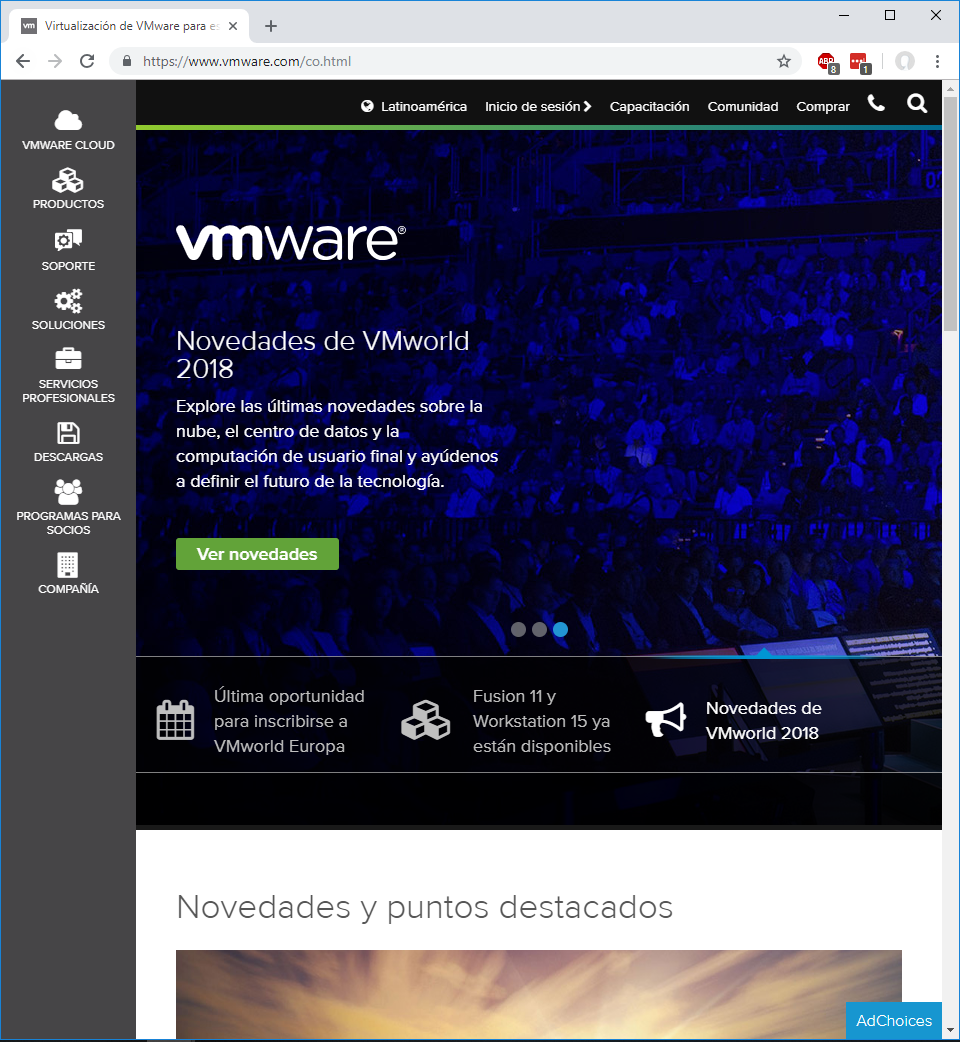
\includegraphics[width=\linewidth]{RE01_VMwareESXi/RE_VMwareInstalacion01.png}
	\vspace{-0.2cm}
	\caption{Sitio web WMWare \url{www.vmware.com}.\footnotemark[2]{} }
	\label{fig:VMwareInstalacion01}
\end{figure}

\footnotetext[2]{La imagen corresponde a la captura de pantalla del sitio web \url{www.vmware.com}.}


\subsubsection{Instalación de VMware ESXi}

Para la instalación de VMWare ESXi es necesario tener la imagen del hipervisor, la cual puede ser obtenido desde la página oficial de VMWare, En la imagen se puede observar que se pueden descargar las diferentes versiones del VMWare ESXi, en el presente trabajo se trabaja con la versión 6.7.
Para la instalación se utilizó una máquina virtual con 8 GB de memoria RAM, un procesador Intel Core i7 6700-HQ y un disco duro de 100GB. Se debe tener la imagen en una memoria flash booteable o en un DVD. Al iniciar el sistema se debe seleccionar el arranque desde la memoria o el DVD y seleccionar como medio el SO VMWare ESXi como se puede observar en la figura \ref{fig:VMwareInstalacion02}.

\begin{figure}[!hbtp]
	\centering
	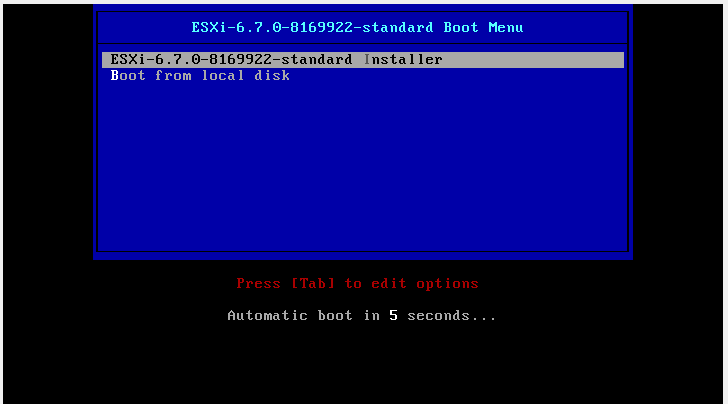
\includegraphics[width=\linewidth]{RE01_VMwareESXi/RE_VMwareInstalacion02.png}
	\vspace{-0.2cm}
	\caption{Sitio Web WMWare \url{www.vmware.com}.\footnotemark[2]{} }
	\label{fig:VMwareInstalacion02}
\end{figure}

El sistema operativo comienza su carga en la memoria, tal como se ve en la imagen.


\begin{figure}[!hbtp]
	\centering
	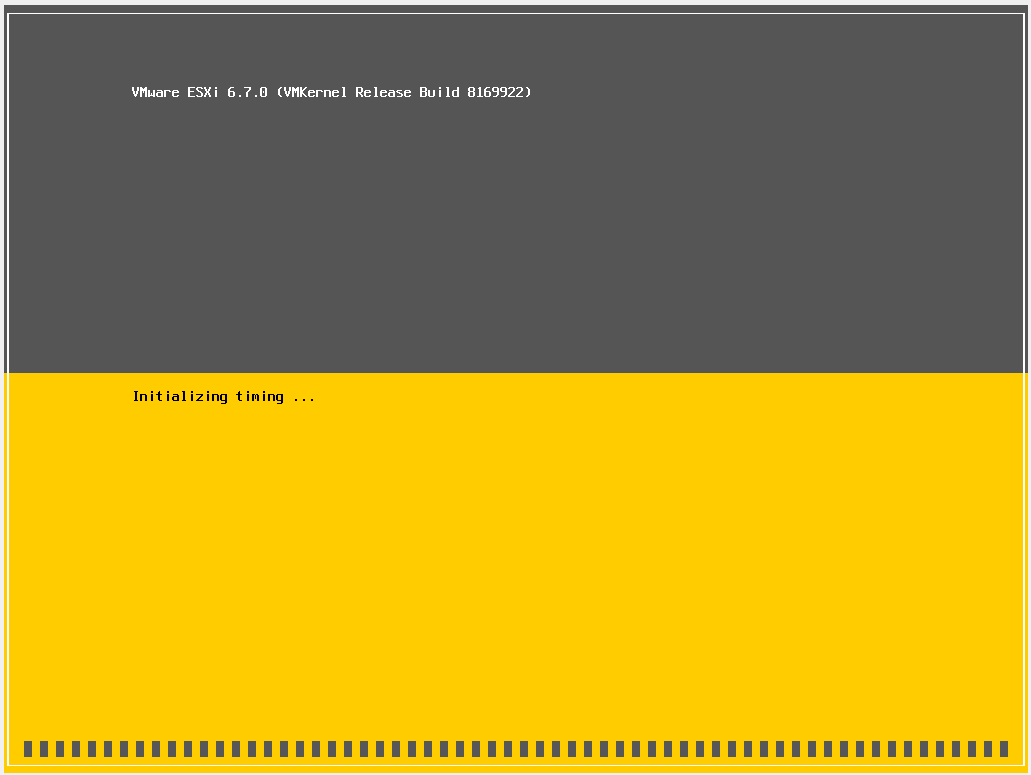
\includegraphics[width=\linewidth]{RE01_VMwareESXi/RE_VMwareInstalacion03.png}
	\vspace{-0.2cm}
	\caption{Sitio Web WMWare \url{www.vmware.com}.\footnotemark[2]{} }
	\label{fig:VMwareInstalacion03}
\end{figure}

\begin{figure}[!hbtp]
	\centering
	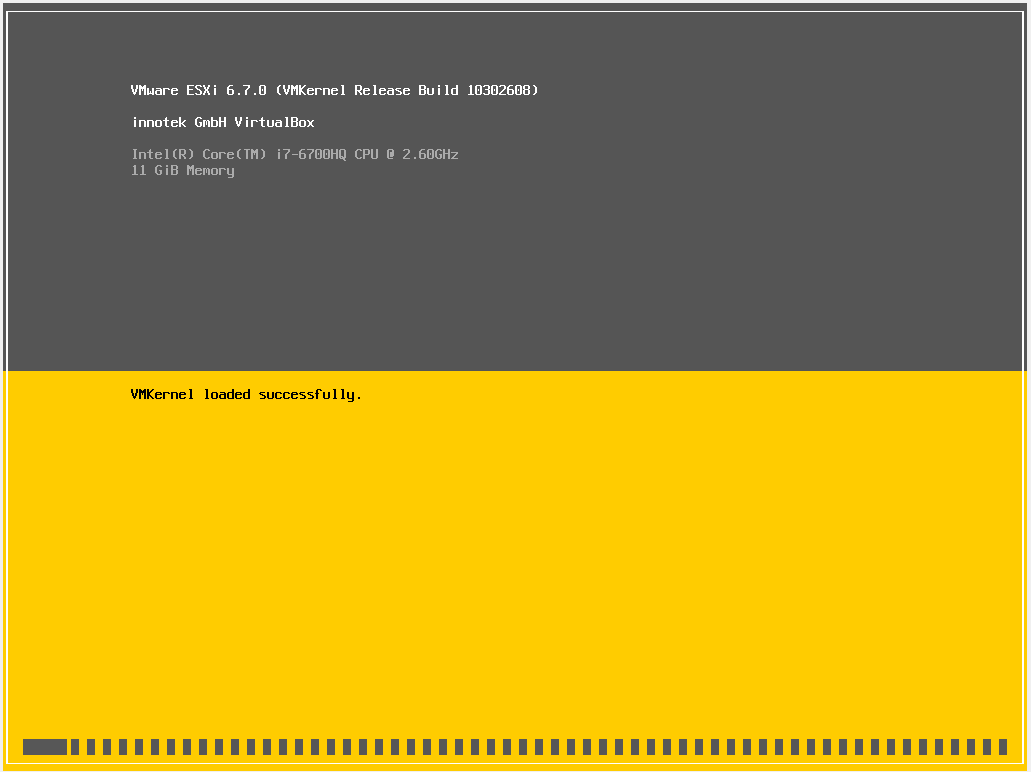
\includegraphics[width=\linewidth]{RE01_VMwareESXi/RE_VMwareInstalacion04.png}
	\vspace{-0.2cm}
	\caption{Sitio Web WMWare \url{www.vmware.com}.\footnotemark[2]{} }
	\label{fig:VMwareInstalacion04}
\end{figure}

\begin{figure}[!hbtp]
	\centering
	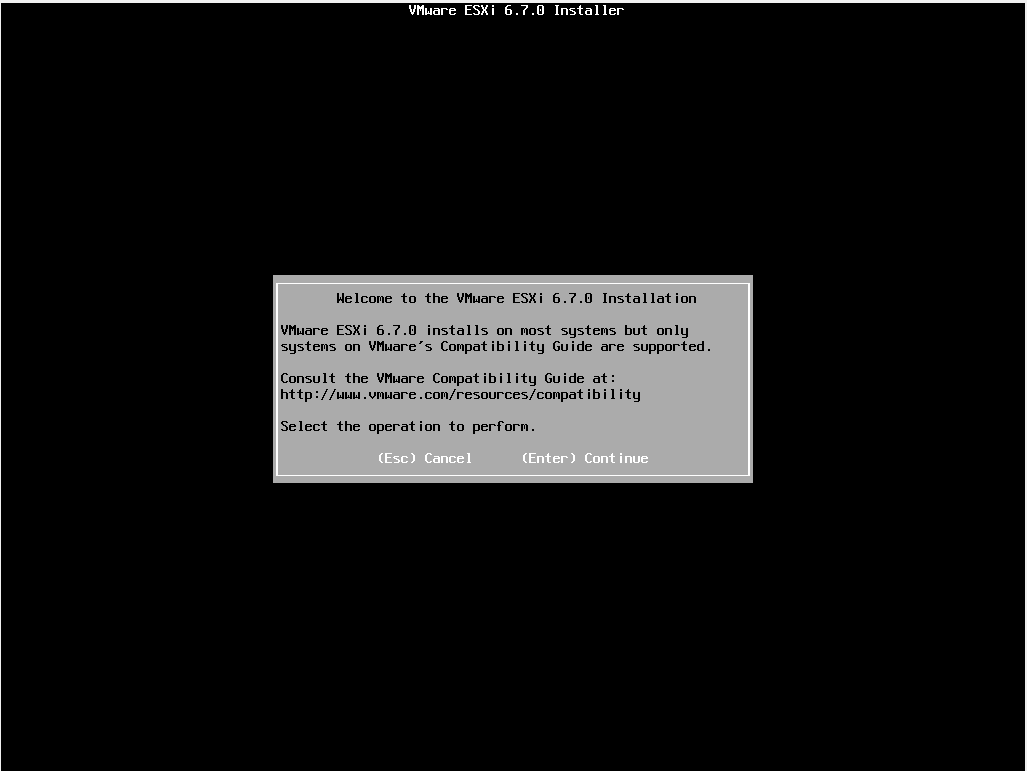
\includegraphics[width=\linewidth]{RE01_VMwareESXi/RE_VMwareInstalacion05.png}
	\vspace{-0.2cm}
	\caption{Sitio Web WMWare \url{www.vmware.com}.\footnotemark[2]{} }
	\label{fig:VMwareInstalacion05}
\end{figure}

\begin{figure}[!hbtp]
	\centering
	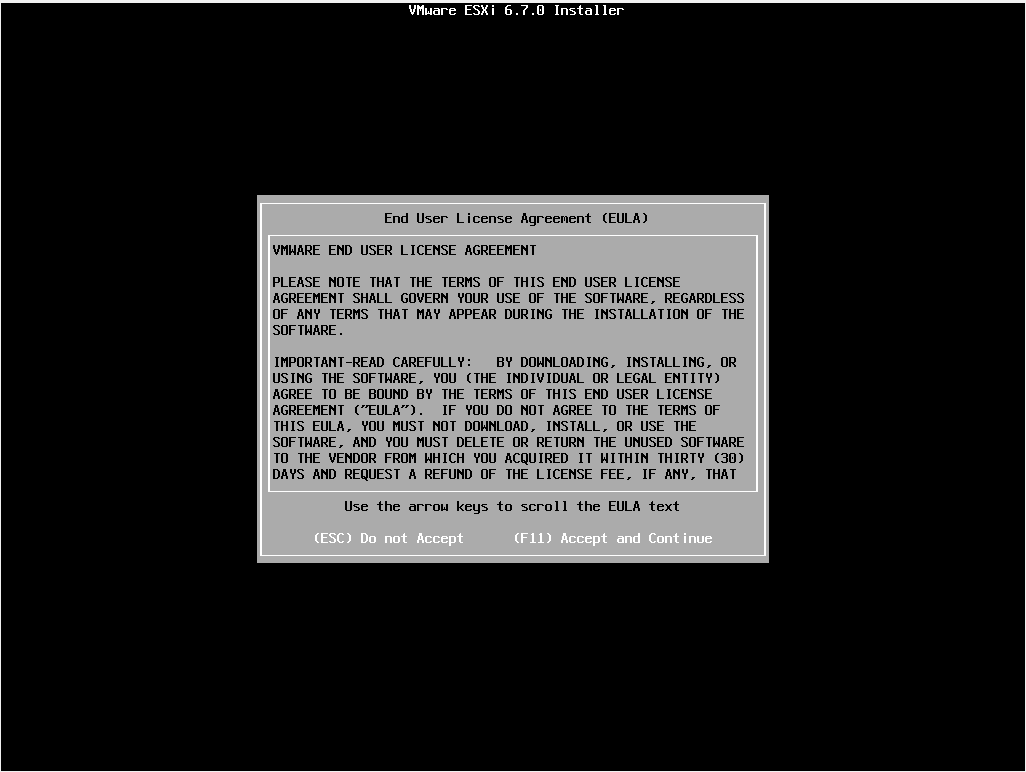
\includegraphics[width=\linewidth]{RE01_VMwareESXi/RE_VMwareInstalacion06.png}
	\vspace{-0.2cm}
	\caption{Sitio Web WMWare \url{www.vmware.com}.\footnotemark[2]{} }
	\label{fig:VMwareInstalacion06}
\end{figure}


\begin{figure}[!hbtp]
	\centering
	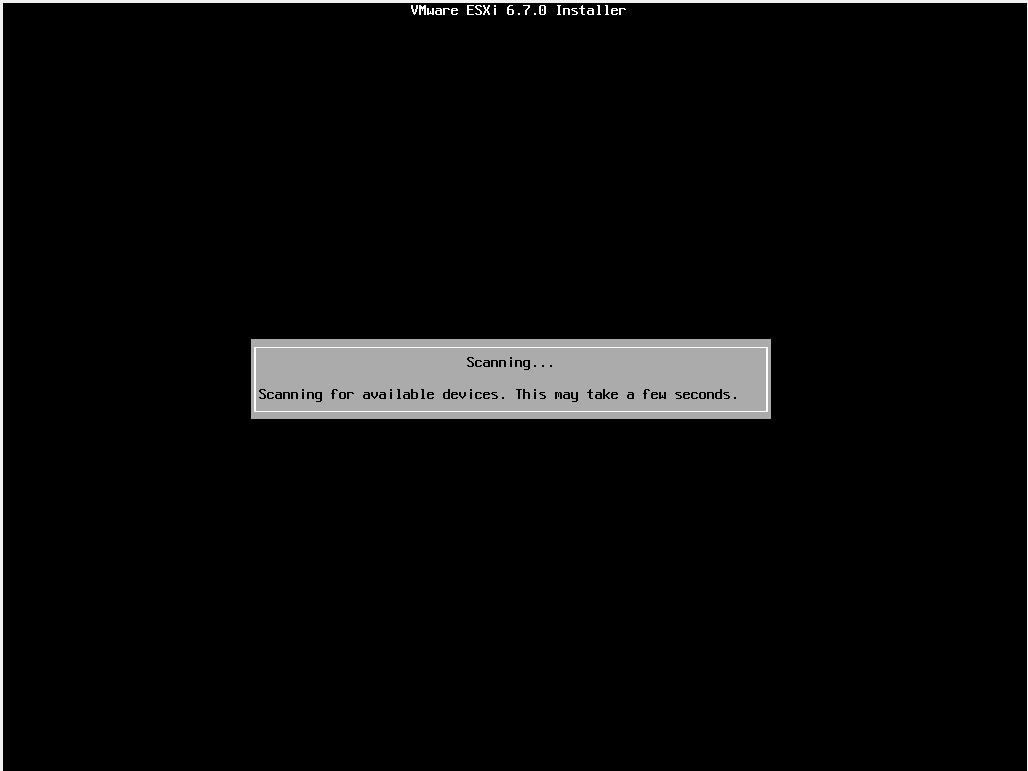
\includegraphics[width=\linewidth]{RE01_VMwareESXi/RE_VMwareInstalacion07.png}
	\vspace{-0.2cm}
	\caption{Sitio Web WMWare \url{www.vmware.com}.\footnotemark[2]{} }
	\label{fig:VMwareInstalacion07}
\end{figure}


\begin{figure}[!hbtp]
	\centering
	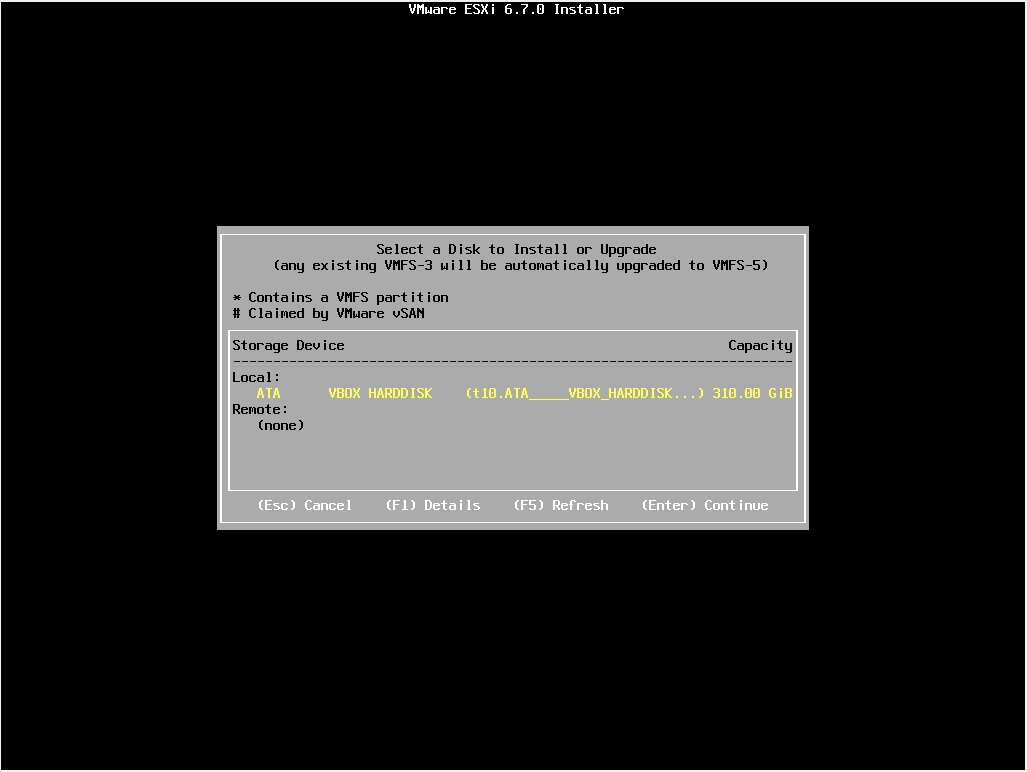
\includegraphics[width=\linewidth]{RE01_VMwareESXi/RE_VMwareInstalacion08.png}
	\vspace{-0.2cm}
	\caption{Sitio Web WMWare \url{www.vmware.com}.\footnotemark[2]{} }
	\label{fig:VMwareInstalacion08}
\end{figure}


\begin{figure}[!hbtp]
	\centering
	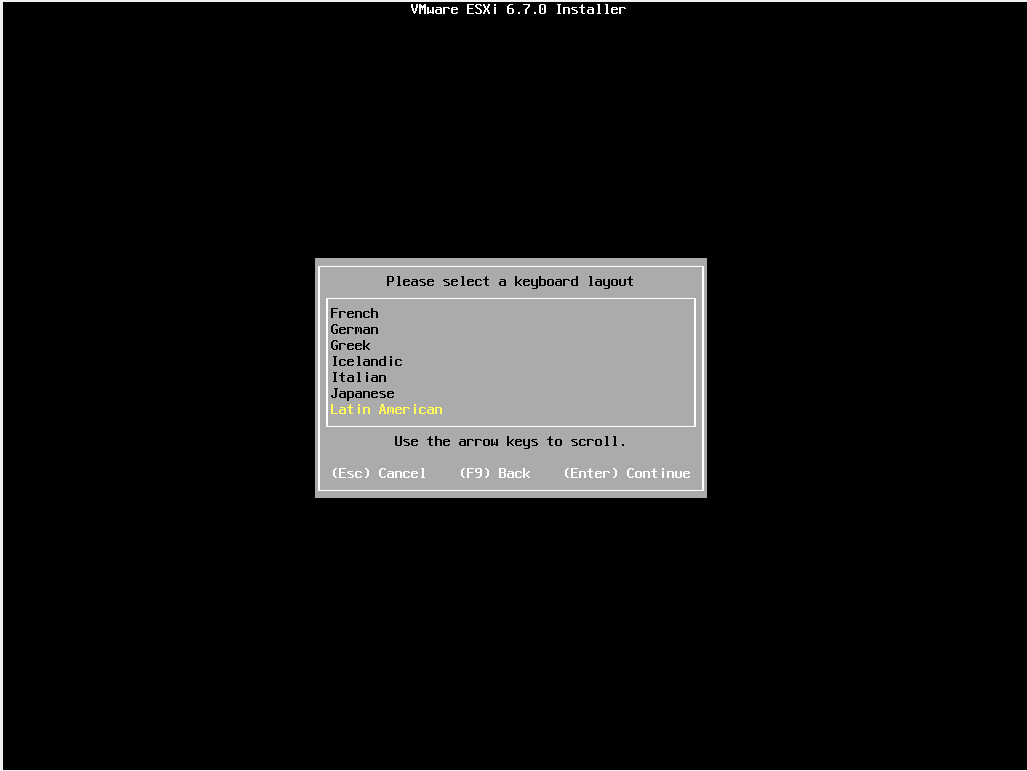
\includegraphics[width=\linewidth]{RE01_VMwareESXi/RE_VMwareInstalacion09.png}
	\vspace{-0.2cm}
	\caption{Sitio Web WMWare \url{www.vmware.com}.\footnotemark[2]{} }
	\label{fig:VMwareInstalacion09}
\end{figure}


\begin{figure}[!hbtp]
	\centering
	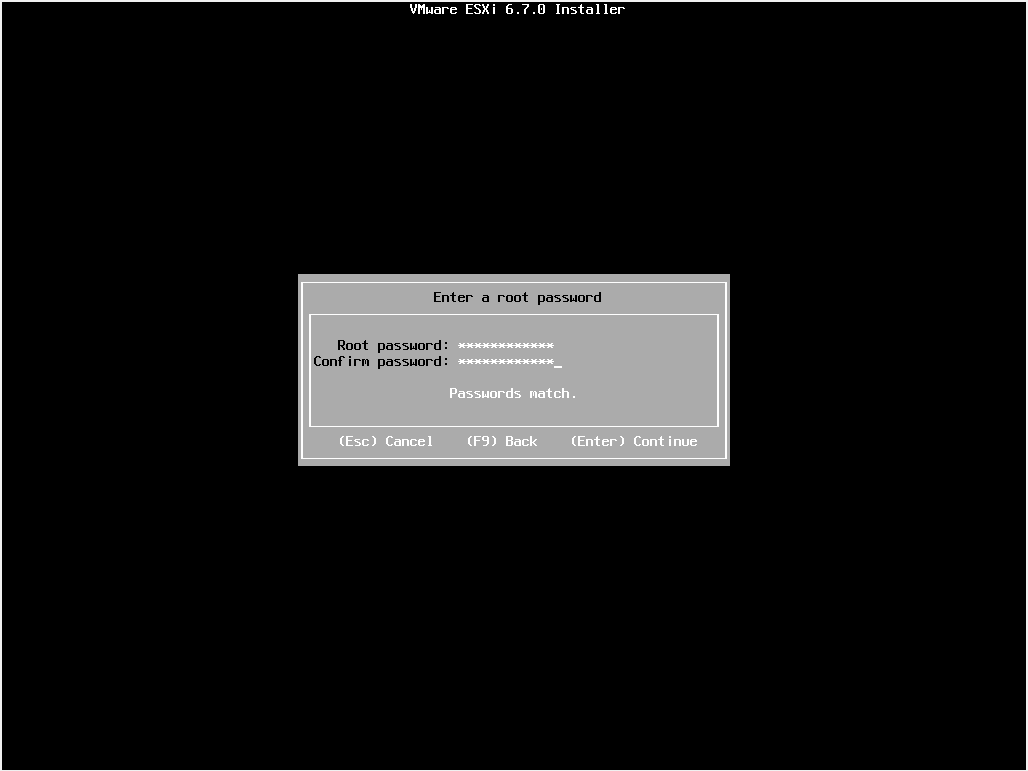
\includegraphics[width=\linewidth]{RE01_VMwareESXi/RE_VMwareInstalacion10.png}
	\vspace{-0.2cm}
	\caption{Sitio Web WMWare \url{www.vmware.com}.\footnotemark[2]{} }
	\label{fig:VMwareInstalacion10}
\end{figure}


\begin{figure}[!hbtp]
	\centering
	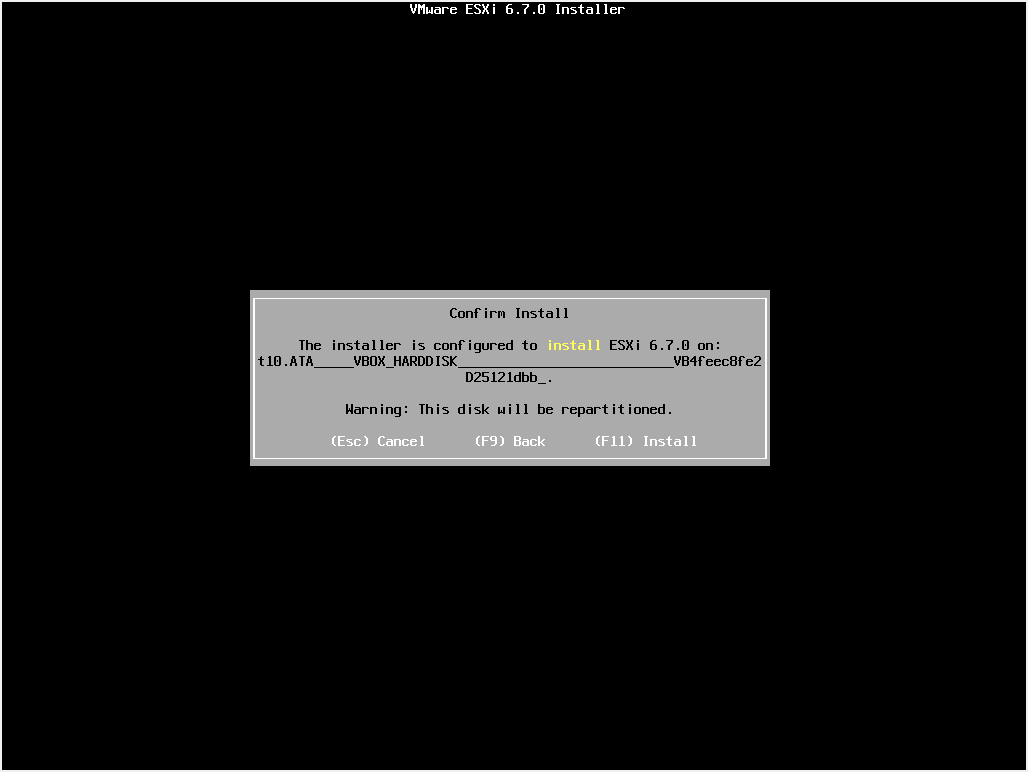
\includegraphics[width=\linewidth]{RE01_VMwareESXi/RE_VMwareInstalacion11.png}
	\vspace{-0.2cm}
	\caption{Sitio Web WMWare \url{www.vmware.com}.\footnotemark[2]{} }
	\label{fig:VMwareInstalacion11}
\end{figure}


\begin{figure}[!hbtp]
	\centering
	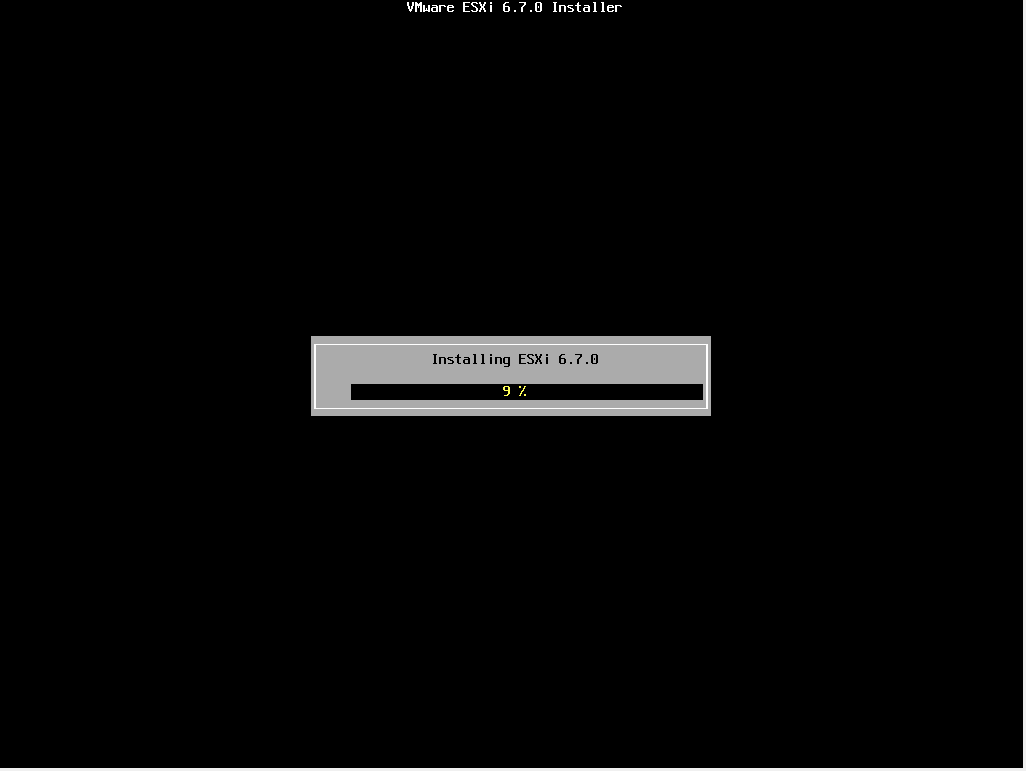
\includegraphics[width=\linewidth]{RE01_VMwareESXi/RE_VMwareInstalacion12.png}
	\vspace{-0.2cm}
	\caption{Sitio Web WMWare \url{www.vmware.com}.\footnotemark[2]{} }
	\label{fig:VMwareInstalacion12}
\end{figure}


\begin{figure}[!hbtp]
	\centering
	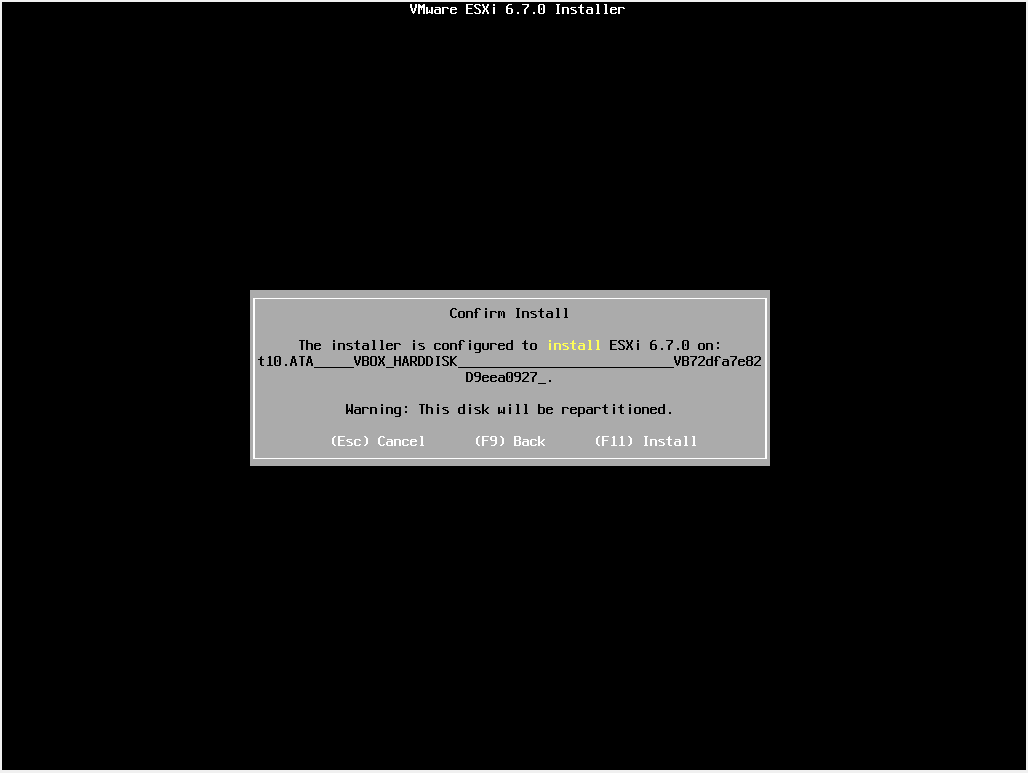
\includegraphics[width=\linewidth]{RE01_VMwareESXi/RE_VMwareInstalacion13.png}
	\vspace{-0.2cm}
	\caption{Sitio Web WMWare \url{www.vmware.com}.\footnotemark[2]{} }
	\label{fig:VMwareInstalacion13}
\end{figure}


\begin{figure}[!hbtp]
	\centering
	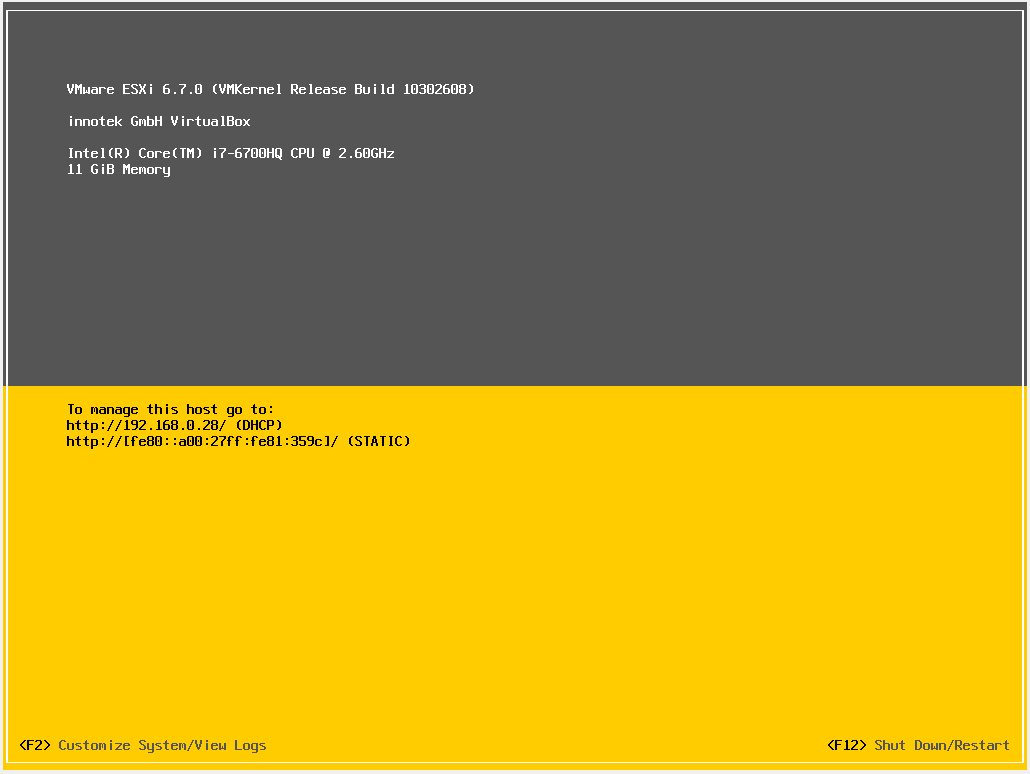
\includegraphics[width=\linewidth]{RE01_VMwareESXi/RE_VMwareInstalacion14.png}
	\vspace{-0.2cm}
	\caption{Sitio Web WMWare \url{www.vmware.com}.\footnotemark[2]{} }
	\label{fig:VMwareInstalacion14}
\end{figure}


\begin{figure}[!hbtp]
	\centering
	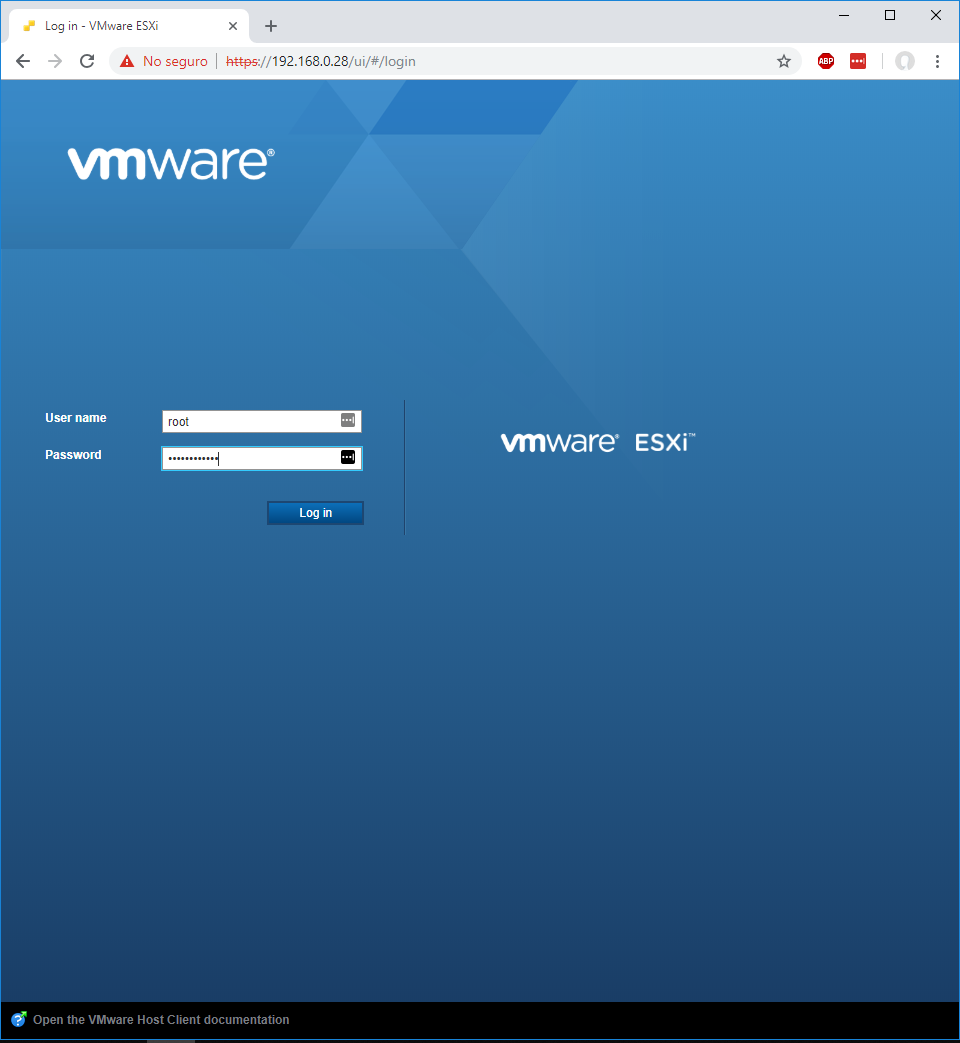
\includegraphics[width=\linewidth]{RE01_VMwareESXi/RE_VMwareInstalacion15.png}
	\vspace{-0.2cm}
	\caption{Sitio Web WMWare \url{www.vmware.com}.\footnotemark[2]{} }
	\label{fig:VMwareInstalacion15}
\end{figure}

\begin{figure}[!hbtp]
	\centering
	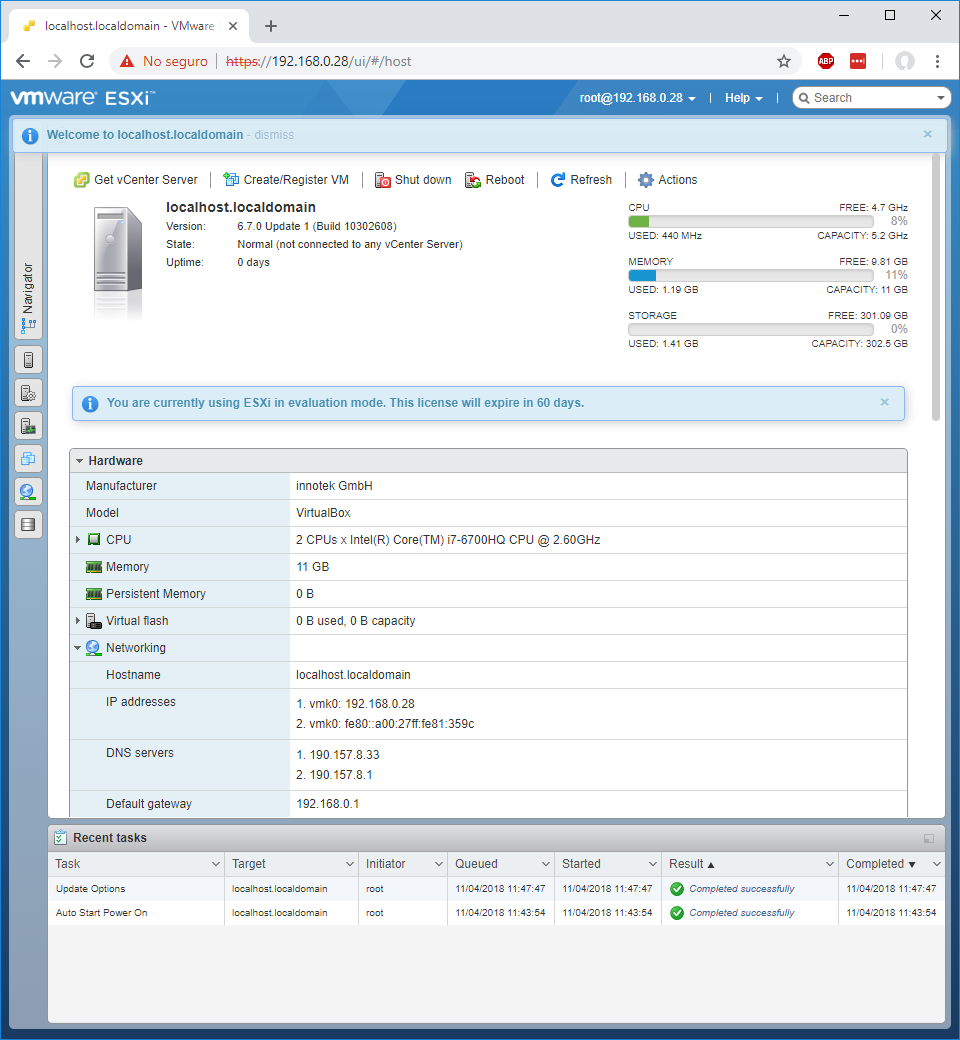
\includegraphics[width=\linewidth]{RE01_VMwareESXi/RE_VMwareInstalacion16.png}
	\vspace{-0.2cm}
	\caption{Sitio Web WMWare \url{www.vmware.com}.\footnotemark[2]{} }
	\label{fig:VMwareInstalacion16}
\end{figure}

\subsubsection{Instalación de VCenter}

Para la instalación de una versión de prueba de VCenter es necesario tener la ISO del appliance, la cual se puede descargar de la página oficial de VMWare como se muestra en la siguiente imagen.



